\documentclass[]{article}
%
\usepackage[T1]{fontenc}
% T1 fonts will be used to generate the final print and online PDFs,
% so please use T1 fonts in your manuscript whenever possible.
% Other font encondings may result in incorrect characters.
%
\usepackage{graphicx}
\usepackage{tabularborder}
\usepackage{booktabs}
\usepackage{tabularx}
\usepackage{float}
\usepackage{tikz}
\usepackage{placeins}
\usepackage{caption}
\usetikzlibrary{shapes}
\usetikzlibrary{fit}
\usepackage{fancyhdr}
\pagestyle{fancy}
\fancyhf{}
\renewcommand{\headrulewidth}{0pt}
\renewcommand{\footrulewidth}{0pt}
\fancyfoot[C]{\thepage}
\usepackage{graphicx} % Para incluir imágenes
\usepackage{amsmath}  % Para matemáticas
\usepackage{pgfplots}
\usepackage{float}
\pgfplotsset{compat=1.16}
\title{\textbf{Proyecto de Simulación: Masa y Resorte}}
\author{Lucio Mansilla , Brenda Dichiara}
\date{\today}

\begin{document}

\maketitle

\section{Introducción}
En este proyecto, exploramos la dinámica de un sistema masa-resorte, con el objetivo de comprender cómo las condiciones iniciales y los parámetros del sistema afectan su comportamiento. Utilizamos el método de Euler para resolver numéricamente las ecuaciones diferenciales que describen el sistema. En este trabajo se observo cómo la masa, la constante del resorte, la resistencia al rozamiento y una fuerza externa aplicada al modelo, afectan a la posición, velocidad oscilaciones, discipación de energía y puntos de equlibrio a lo largo del tiempo.

\section{Modelo y Método de Solución}
El modelo físico que utilizamos es el de un resorte con una masa $m$ sujeta a él, una constante de resistencia del resorte $k$, una resistencia al rozamiento $b$, y una fuerza externa $F$.

\vspace{0.1cm}
\begin{center}
\begin{tikzpicture}[scale=1.5]

    % Masa
    \draw[fill=white,opacity=0.7] (2,-0.5) rectangle ++(1,1) node[midway] {$m$};
    % Resorte
    \draw[decoration={coil},decorate] (0,0) -- (2,0) node[midway, above=5mm] {$k$};
    % Pared
    \draw[very thick] (0,-1) -- (0,1);
    % Fuerza
    \draw[->,thick, red] (3,0) -- ++(1,0) node[midway,above] {$F(t)$};
    % Rozamiento
    \draw[->,thick, blue] (2,-0.5) -- ++(-0.5,0) node[midway,below] {$b$};
    % Coordenadas
    \draw[->] (0,-1) -- ++(5,0) node[below] {$x(t)$}; % posicion
    \draw[->] (0,-1) -- ++(0,2) node[left] {$y(t)$}; % velocidad
\end{tikzpicture}
\end{center}
Las ecuaciones diferenciales que modelan este sistema continuo son:
\begin{align*}
    \frac{dx}{dt} & = v \\\\ 
    \frac{dv}{dt} & = -\frac{k}{m}x - \frac{b}{m}v + \frac{F}{m}.
\end{align*}

\section{Validación del Modelo}
Para validar el modelo de simulación de masa-resorte, necesitamos comparar los resultados de la simulación con los resultados experimentales o con soluciones analíticas conocidas del sistema.

\subsection{Comparación con Soluciones Analíticas}
% La ecuación diferencial que describe un sistema masa-resorte sin amortiguamiento es una ecuación bien conocida cuya solución es una función sinusoidal o cosinusoidal. Si incluimos el amortiguamiento, la solución se convierte en una exponencial amortiguada multiplicada por una sinusoidal o cosinusoidal. Podemos comparar los resultados de nuestra simulación con estas soluciones analíticas para verificar que nuestro modelo esté funcionando correctamente. 


\section{Experimentos}
Realizamos una serie de experimentos variando la masa $m$, la constante del resorte $k$, la resistencia al rozamiento $b$, la fuerza externa $F$, y las condiciones iniciales de posición  , velocidad $x_0$ ,$v_0$ y el "paso" de tiempo $\Delta t$. A continuación, presentamos los resultados más interesantes de estos experimentos.

\subsection{Experimento 1: Variación de la masa}
En este experimento, nos centramos en el impacto en  la variación de la masa $m$ en la dinámica del sistema. Para asegurar un control riguroso sobre las variables de estudio, mantuvimos constantes el resto de los parámetros:

\begin{itemize}
\item Constante del resorte, $k = 1.0$
\item Resistencia al rozamiento, $b = 1.0$
\item Fuerza externa, $F = 1.0$
\item Posición inicial, $x_0 = 0.0$
\item Velocidad inicial, $v_0 = 0.0$
\end{itemize}

Luego, implementamos simulaciones con distintos valores de masa, en particular $m = 1.0$ y $m = 3.0$. El paso de tiempo seleccionado para la simulación fue $\Delta t= 0.001$.

Las simulaciones realizadas con 150 como límite de tiempo $t$ mostraron que a medida que la masa aumenta, el sistema tarda un mayor tiempo en alcanzar un estado de equilibrio, como se puede ver en la figura 1.


\captionsetup[figure]{
  font=small,
  labelfont=bf,
  margin={1cm,0cm}
}

\begin{figure}[H]
\centering
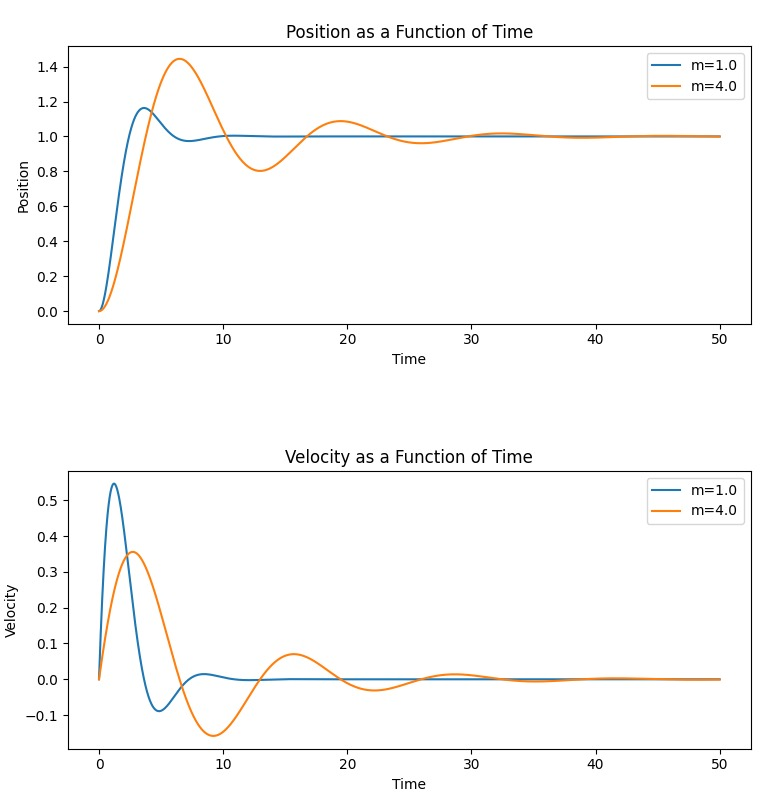
\includegraphics[width=\textwidth]{../assets/figure_1_mass.jpeg}
\caption{Posición - Velocidad en función del tiempo para distintos valores de masa, $t = 100$.}
\end{figure}


Este fenómeno se debe a que la fuerza aplicada, es constante i.e $F = 1$, por lo que se necesita más tiempo para generar suficiente impulso y mover la masa aumentada hacia el estado de equilibrio. Notar que en este caso al ser $t$ un límite de tiempo bajo, el sistema con mayor masa produce menos oscilaciones, puesto que la velocidad es menor y la amplitud es mayor, es decir, alcanza valores más altos en cuanto a posición lejos del equilibrio.\\

Mismo experimento pero aumentando el límite de tiempo 
$t$ mostro que el modelo con mayor masa presenta más oscilaciones antes de alcanzar el estado de equilibrio, como se puede ver en la figura 2.

\begin{figure}[H]
    \centering
    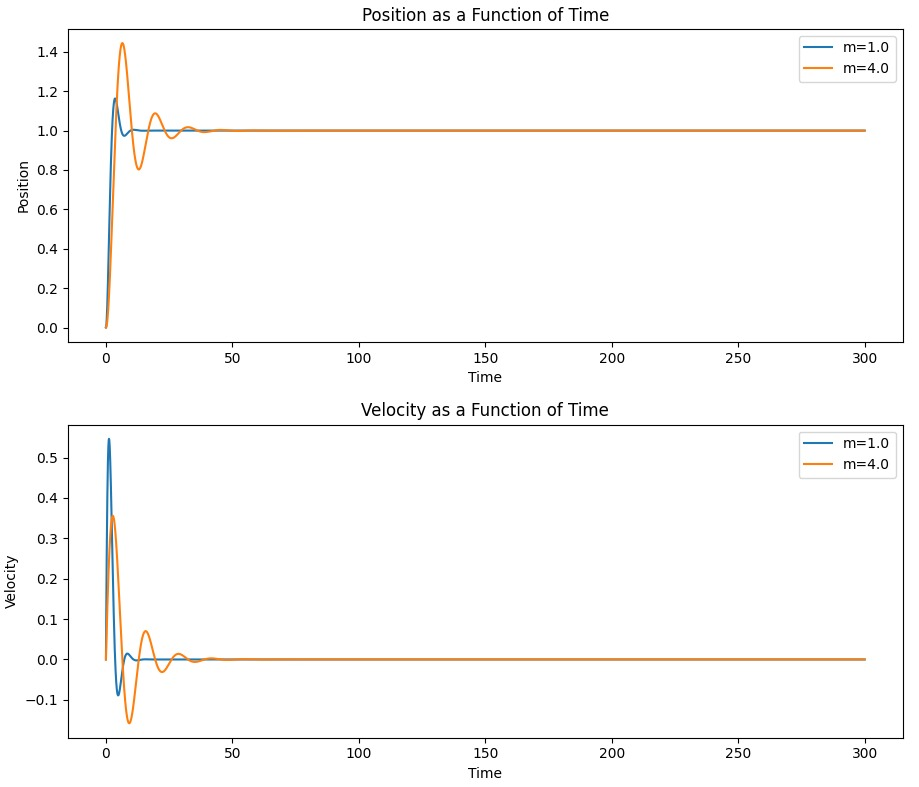
\includegraphics[width=\textwidth]{../assets/figure_3_mass.jpeg}
    \caption{Posición - Velocidad en función del tiempo para distintos valores de masa, $t = 150$.}
\end{figure}
    

Se presentan los resultados observados de la figura 1 y 2 junto con los datos de oscilacion, velocidad y posición en las tablas 1 2 y 3.
\captionsetup[table]{
  font=small,
  labelfont=bf,
  margin={1cm, 0cm}
}

\begin{table}[H]
    \caption{Resultados de la variación de la masa, el tiempo y las oscilaciones}
    \label{tab:mass_time_oscillations}
    \centering
    \begin{tabular*}{\textwidth}{@{\extracolsep{\fill}}|c|c|c|}
    \hline
    \textbf{Masa ($m$)} & \textbf{Tiempo Lim. ($t$)} & \textbf{Oscilaciones} \\
    \hline
    1.0 & 50 & 13 \\
    \hline
    4.0 & 50 & 7 \\
    \hline
    1.0 & 300 & 16 \\
    \hline
    4.0 & 300 & 36 \\
    \hline
    \end{tabular*}
\end{table}

\begin{table}[H]
    \caption{Resultados de la variación de la masa, el tiempo y la velocidad}
    \label{tab:mass_time_velocity}
    \centering
    \begin{tabular*}{\textwidth}{@{\extracolsep{\fill}}|c|c|c|c|}
    \hline
    \textbf{Masa ($m$)} & \textbf{Tiempo Lim. ($t$)} & \textbf{Vel. Máx.} & \textbf{Vel. Mín.} \\
    \hline
    1.0 & 50 & 0.546 & -0.089 \\
    \hline
    4.0 & 50 & 0.356 & -0.158 \\
    \hline
    1.0 & 300 & 0.546 & -0.089 \\
    \hline
    4.0 & 300 & 0.356 & -0.158 \\
    \hline
    \end{tabular*}
\end{table}

\begin{table}[H]
    \caption{Resultados de la variación de la masa, el tiempo y la posición}
    \label{tab:mass_time_position}
    \centering
    \begin{tabular*}{\textwidth}{@{\extracolsep{\fill}}|c|c|c|c|}
    \hline
    \textbf{Masa ($m$)} & \textbf{Tiempo Lim. ($t$)} & \textbf{Pos. Máx.} & \textbf{Pos. Mín.} \\
    \hline
    1.0 & 50 & 1.163 & 0 \\
    \hline
    4.0 & 50 & 1.444 & 0 \\
    \hline
    1.0 & 300 & 1.163 & 0 \\
    \hline
    4.0 & 300 & 1.444 & 0 \\
    \hline
    \end{tabular*}
\end{table}
A partir de los datos presentados en las tablas, se puede observar que el sistema con una mayor masa (4.0) presenta un mayor número de oscilaciones, una velocidad máxima y mínima más baja, y una mayor posición máxima en comparación con el sistema con una masa más baja (1.0). Esto refuerza la observación de que el sistema con una mayor masa tarda más tiempo en alcanzar el equilibrio y tiene una mayor amplitud de oscilación.

\subsection{Experimento 2: Ausencia de Fricción}

En este experimento, exploramos la dinámica del sistema en ausencia de fricción. Específicamente, comparamos dos modelos con las siguientes características:

\begin{itemize}
\item Modelo 1: $m = 1.0$, $k = 1.0$, $b = 1.0$, $F = 1.0$
\item Modelo 2: $m = 1.0$, $k = 1.0$, $b = 0.0$, $F = 1.0$
\end{itemize}

Ejecutamos simulaciones para ambos modelos con un tiempo de simulación de $t = 300$ y un paso de tiempo $\Delta t = 0.001$. 

Los resultados para el modelo 1, con fricción, se resumen en la tabla 4.

\begin{table}[H]
    \caption{Resultados para el Modelo 1 con fricción}
    \label{tab:model_1_friction}
    \centering
    \begin{tabular*}{\textwidth}{@{\extracolsep{\fill}}|c|c|c|c|}
    \hline
    \textbf{Oscilaciones} & \textbf{Vel. Máx.} & \textbf{Vel. Mín.} & \textbf{Pos. Máx.} \\
    \hline
    16 & 0.546 & -0.089 & 1.163 \\
    \hline
    \end{tabular*}
\end{table}

Los resultados para el modelo 2, sin fricción, se resumen en la tabla 5.

\begin{table}[H]
    \caption{Resultados para el Modelo 2 sin fricción}
    \label{tab:model_2_no_friction}
    \centering
    \begin{tabular*}{\textwidth}{@{\extracolsep{\fill}}|c|c|c|c|}
    \hline
    \textbf{Oscilaciones} & \textbf{Vel. Máx.} & \textbf{Vel. Mín.} & \textbf{Pos. Máx.} \\
    \hline
    95 & 1.000 & -1.000 & 2.000 \\
    \hline
    \end{tabular*}
\end{table}

Los resultados muestran que en ausencia de fricción, el sistema realiza más oscilaciones (95 en lugar de 16), alcanza velocidades más altas (máximo de 1.000 en lugar de 0.546), y alcanza posiciones más alejadas del equilibrio (máximo de 2.000 en lugar de 1.163).

Repetimos las simulaciones para un tiempo de simulación más corto, $t = 100$, y observamos resultados consistentes con el tiempo de simulación más largo.

En general, estos resultados destacan el papel crítico de la fricción en la amortiguación de las oscilaciones, la limitación de las velocidades máximas y la restricción de las posiciones máximas que el sistema puede alcanzar.

\subsection{Experimento 3: Desplazamiento del estado de equilibrio}

En este experimento, investigamos el efecto de variar la fuerza $F$ en la dinámica del sistema. Mantuvimos los demás parámetros constantes, es decir:

\begin{itemize}
\item Masa, $m = 1.0$
\item Constante del resorte, $k = 1.0$
\item Resistencia al rozamiento, $b = 1.0$
\item Posición inicial, $x_0 = 0.0$
\item Velocidad inicial, $v_0 = 0.0$
\end{itemize}

Luego, implementamos simulaciones con distintos valores de fuerza, en particular $F = 1.0$, $F = 2.0$ y $F = 3.0$. 

Los resultados de las simulaciones para cada valor de fuerza se resumen en la tabla 6.

\begin{table}[H]
    \caption{Resultados para distintos valores de fuerza}
    \label{tab:force_results}
    \centering
    \begin{tabular*}{\textwidth}{@{\extracolsep{\fill}}|c|c|c|c|c|}
    \hline
    \textbf{Fuerza ($F$)} & \textbf{Oscilaciones} & \textbf{Vel. Máx.} & \textbf{Vel. Mín.} & \textbf{Pos. Máx.} \\
    \hline
    1.0 & 13 & 0.546 & -0.089 & 1.163 \\
    \hline
    2.0 & 13 & 1.093 & -0.178 & 2.326 \\
    \hline
    3.0 & 13 & 1.639 & -0.267 & 3.489 \\
    \hline
    \end{tabular*}
\end{table}

Los resultados muestran que aumentar la fuerza aplicada aumenta tanto la velocidad máxima como la posición máxima alcanzada por el sistema, sin alterar el número de oscilaciones.

El efecto de la variación de la fuerza se puede visualizar en la figura 3, que muestra la posición y la velocidad en función del tiempo para los distintos valores de fuerza.

\captionsetup[figure]{
  font=small,
  labelfont=bf,
  margin={1cm,0cm}
}

\begin{figure}[H]
\centering
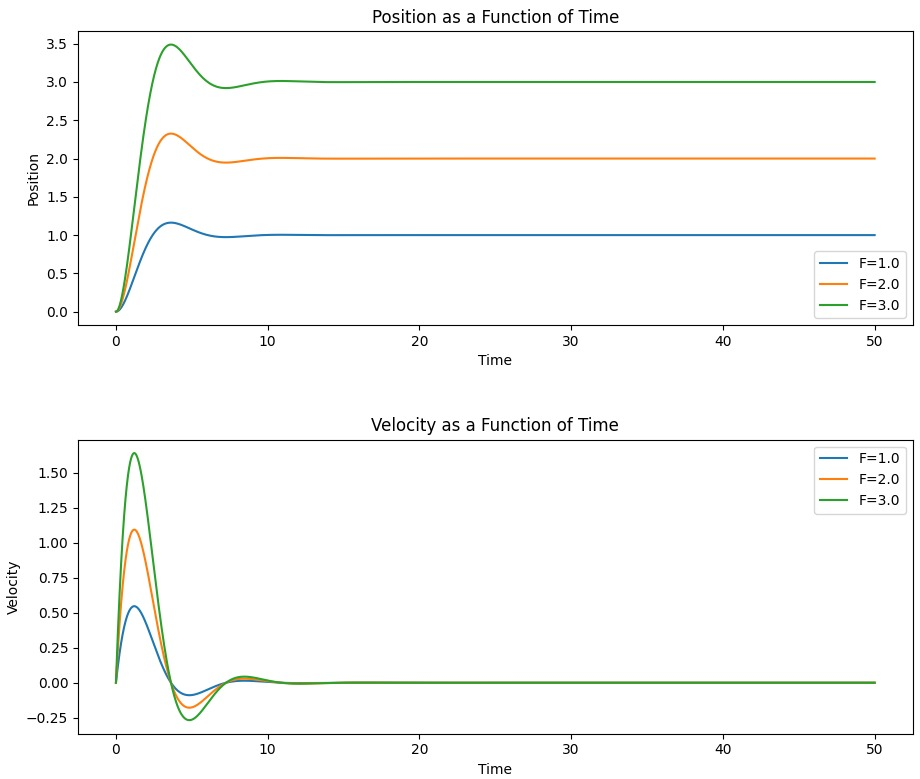
\includegraphics[width=\textwidth]{../assets/figure_1_force.jpeg}
\caption{Posición - Velocidad en función del tiempo para distintos valores de fuerza.}
\end{figure}

Estos resultados indican que aumentar la fuerza aplicada al sistema puede ser una forma efectiva de aumentar tanto la velocidad como la distancia que el sistema puede alcanzar sin alterar significativamente la frecuencia de oscilación.

\section{Conclusiones}
Conclusiones basadas en los resultados de los experimentos...


\end{document}
